\newpage
\subsection{User Interface Design}
The interaction design foundation defines user interface (UI) design as "the process designers use
to build interfaces in software or computerized devices, focusing on looks or style. Designers aim
to create interfaces which users find easy to use and pleasurable. UI design refers to graphical
user interfaces and other forms—e.g., voice-controlled interfaces."
\directcite{interactiondesignfoundation-ixdfWhatUserInterface2016}.

This definition is a good starting point to understand what UI design is about, since it
shows that it is about more than just the visual. User interfaces are everywhere, be it an ATM, a
stove, a bike computer or a time tracking app in the browser. Each one of them needs to be
carefully designed. It is about finding ways to make this human-computer interaction as smooth,
efficient and delightful as possible.
\vglcite{interactiondesignfoundation-ixdfWhatUserInterface2016}

\subsubsection{Web Design}
Web design is a subset of UI design that specifically focuses on designing websites. While other UI
Design fields often focus on specific platforms, web designers have to consider a wide range of end
user devices like desktop PCs, tablets or smartphones. The practice of adapting and optimizing for
these various screen sizes and aspect ratios is known as \textit{Responsive Design}. Additionally,
\textit{web accessibility} is a fundamental aspect of web design. It ensures that people with
disabilities can navigate and interact with websites as effective as possible.
\vglcite{interactiondesignfoundation-ixdfWhatWebDesign2016}

With the European Accessibility Act (EAA) coming into effect in June 2025, this becomes even more
important, as businesses need to comply with stricter regulations on all of their websites.
\vglcite{kleeAccessibilityAct20252024}

Although web design is often thought of as a purely visual discipline, when in reality it is a much
more multidisciplinary field. Designers have to work closely with developers and often know a great
deal of content strategy, information architecture, user research and more. Product designer Mark
Boulton emphazises that "you can create good experiences without knowing the content. What you can't
do is create good experiences without knowing your content structure. What is your content made
from, not what your content is." \directcite{boultonStructureFirstContent2012}

\subsubsection{User Experience and Usability}
Zooming out of the context of User Interfaces is essential to fully understand the concept of User
Experience (UX). UX is about looking at all kinds of touch-points a user has with a product or
service and seeing the holistic experience. This of course includes the UI, but encompasses several
other domains such as content quality, customer support, branding, and more.
\vglcite{normanDefinitionUserExperience1998}

In other words, even an app like Spotify with a great interface, would have a poor UX if there were
only 10 songs available.

Usability on the other hand is, as Jacob Nielsen suggests, a quality attribute of Interfaces. This
attribute indicates how easy it is for users to use a product, by observing and measuring the five
quality components: learnability, efficiency, memorability, errors, and satisfaction
defined by Nielsen. Additionally, Nielsen introduces another concept that when combined with
usability is an indicator for the overall usefulness of a product - utility. Utility refers to
whether a product offers the necessary features that a user actually needs. Both usability and
utility are crucial for a successful product. Simply having an intuitive interface is of no use if
the product lacks the necessary features. Similarly, a product with a fitting feature-set is
ineffective if users struggle navigating it.
\vglcite{nielsenUsability101Introduction2012}
% NOTE DONE: Potential for graphic here (Vann Diagram)
\begin{figure}[H]
    \centering
    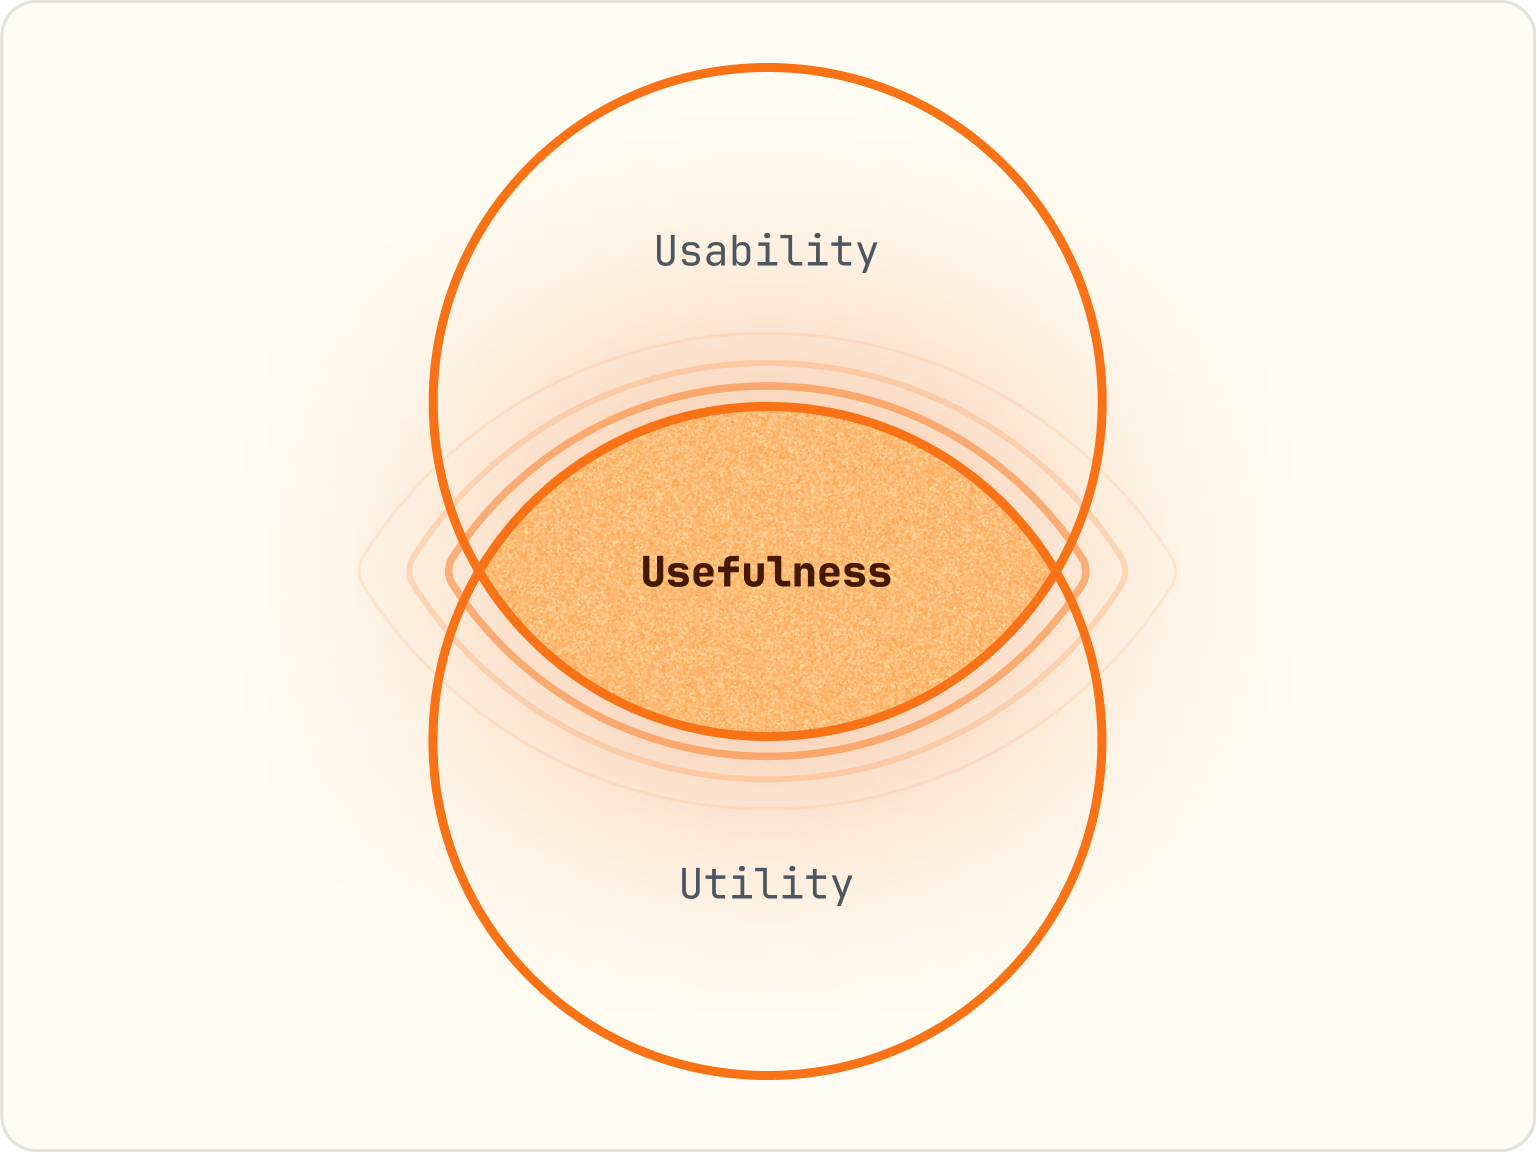
\includegraphics[height=250pt]{Chapter 2/Usefulness.png}
    \caption{Combination of usability and utility according to Jacob Nielsen (Source: own illustration)}
\end{figure}

\subsubsection{Tools}
There are many great tools available that aim to make user interface design easier and more
efficient. Some of them also have features that help to bridge the gap between design and code. The
selection of tools is based on their popularity, since the aim is to provide a solution that
tailors to the majority of designers and developers. % NOTE DONE: Add graphic showing the popularity of
% tools (https://uxtools.co/survey/2023/ui-design/#ui-design-yoy-graph)
\begin{figure}[H]
    \centering
    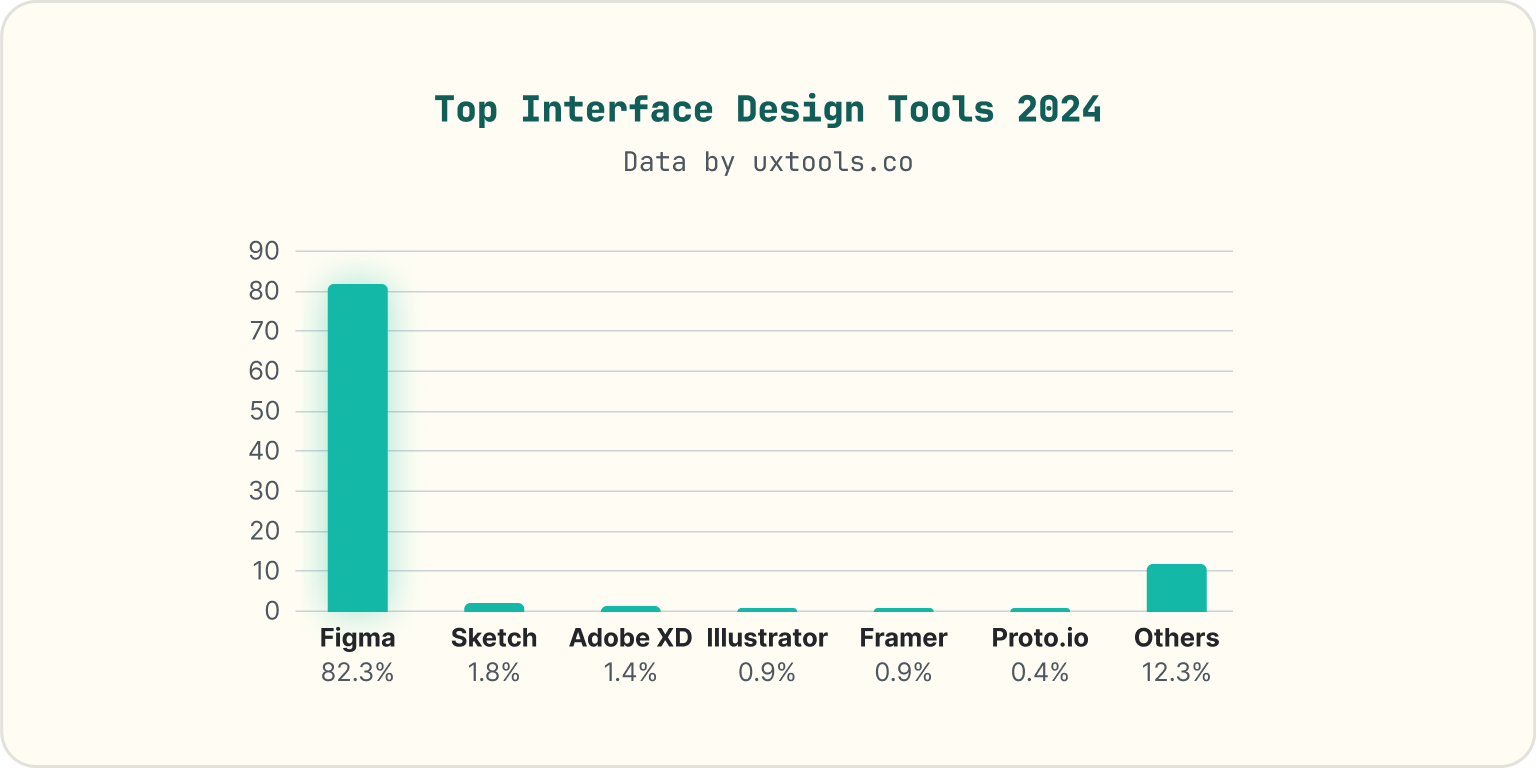
\includegraphics[height=250pt]{Chapter 2/Top Design Tools.png}
    \caption{Top Design Tools (Source: own illustration based on data of UXTools in https://www.uxtools.co/survey/interface-design/overview)}
\end{figure}

% NOTE DONE: Add Logo graphic for each of the tools
\textbf{Figma}\\
\begin{figure}[H]
    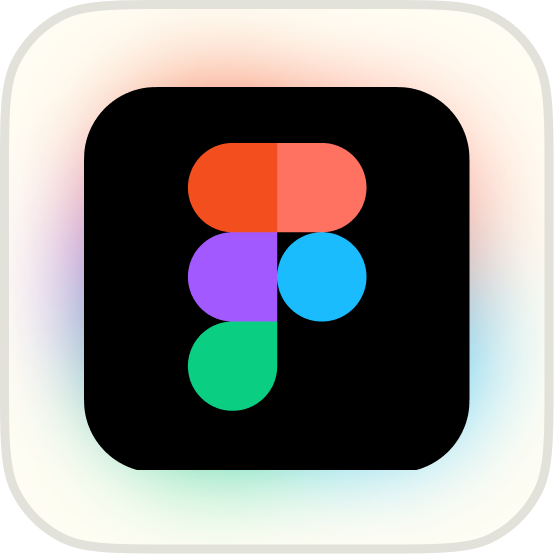
\includegraphics[height=50pt]{Chapter 2/Figma.png}
    \caption{Figma Logo (Source: modified illustration based on Figma in https://www.figma.com/using-the-figma-brand/)}
\end{figure}
According to UXTools yearly survey, Figma is by far the most popular UI design tool at the moment.
\vglcite{uxtools2024DesignTools2024} It is a cloud-based design tool that focuses on real-time
collaboration, prototyping and design system creation. The majority of features is free to use,
which makes it very approachable. Apart from their frequent updates and improvements, Figma has a
lively community allowing for the creation of plugins, templates and other resources. Having robust
design system features like components, style definitions and variables, Figma is one of the leading
tools in the UI design space. \vglcite{figmaFigma}

\textbf{Sketch}\\
\begin{figure}[H]
    
\includegraphics[height=50pt]{Chapter 2/Sketch.png}
    \caption{Sketch Logo (Source: modified illustration based on Sketch in https://www.sketch.com/about-us)}
\end{figure}
Sketch is a design tool that was first released in 2010. Although, Figma has surpassed Sketch in
terms of popularity, it still has a large user base. It offers similar features to Figma like
real-time collaboration, components or prototyping. However, aside from the free, browser-accessible
file viewer, Sketch is a paid tool available only on macOS. The program has a strong focus on
creating design systems and a large library of available plugins and templates. 
\vglcite{sketchSketch}

\textbf{Adobe Illustrator and Adobe Photoshop}\\
\begin{figure}[H]
    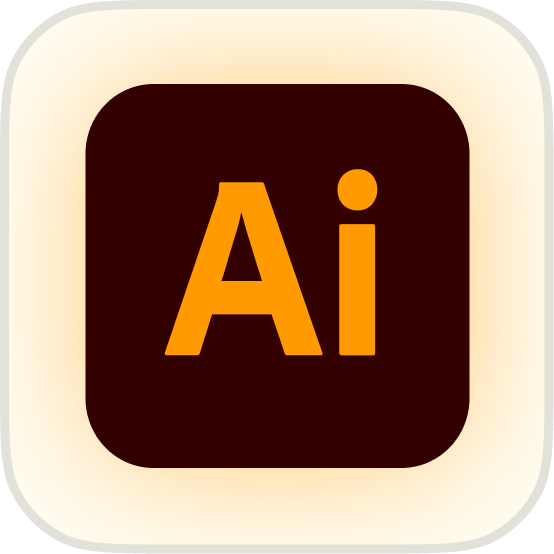
\includegraphics[height=50pt]{Chapter 2/Illustrator.png}
    \caption{Illustrator Logo (Source: modified illustration based on Adobe in https://www.adobe.com/cc-shared/assets/img/product-icons/svg/illustrator.svg)}
\end{figure}
Although the vector graphics editor Adobe Illustrator and the raster graphics editor Adobe Photoshop
are not specifically tailored to UI design, they are widely used by designers. Many designers report
that they use them as secondary tools aiding in the creation of more complex graphics.
\vglcite{uxtools2024DesignTools2024}

In future chapters, the author will generally refer to Figma, since it is the most popular tool at
the moment and also the one the author is most familiar with. Although the majority of concepts and
techniques mentioned will be applicable to other tools as well.
